\documentclass[12pt]{article}

%%%%%%%%%%%%%%%%%%%%%%%%%%%%%%%%%%%%%%%%%%%%%%%%%%%%%%%%%%%%%%%%%%%%%%%%%%%%%%%%%%%%%%%%%%%%%%%%%%%%
% Math
\usepackage{fancyhdr} 
\usepackage{amsfonts}
\usepackage{amsmath}
\usepackage{amssymb}
\usepackage{amsthm}
%\usepackage{dsfont}

%%%%%%%%%%%%%%%%%%%%%%%%%%%%%%%%%%%%%%%%%%%%%%%%%%%%%%%%%%%%%%%%%%%%%%%%%%%%%%%%%%%%%%%%%%%%%%%%%%%%
% Macros
\usepackage{calc}

%%%%%%%%%%%%%%%%%%%%%%%%%%%%%%%%%%%%%%%%%%%%%%%%%%%%%%%%%%%%%%%%%%%%%%%%%%%%%%%%%%%%%%%%%%%%%%%%%%%%
% Commands and Custom Variables	
\newcommand{\problem}[1]{\hspace{-4 ex} \large \textbf{Problem #1} }
%\let\oldemptyset\emptyset
%\let\emptyset\varnothing
\newcommand{\norm}[1]{\left\lVert#1\right\rVert}
\newcommand{\sint}{\text{s}\kern-5pt\int}
\newcommand{\powerset}{\mathcal{P}}
\renewenvironment{proof}{\hspace{-4 ex} \emph{Proof}:}{\qed}
\newcommand{\solution}{\textit{Solution}:\bigbreak}
\newcommand{\RR}{\mathbb{R}}
\newcommand{\NN}{\mathbb{N}}
\newcommand{\QQ}{\mathbb{Q}}
\newcommand{\ZZ}{\mathbb{Z}}
\newcommand{\CC}{\mathbb{C}}
\newcommand{\VV}{\mathbb{V}}
\newcommand{\FF}{\mathbb{F}}
\renewcommand{\Re}{\operatorname{Re}}
\renewcommand{\Im}{\operatorname{Im}}

\newcommand{\bigO}{\mathcal{O}}

\renewcommand{\vec}[1]{\boldsymbol{\mathbf{#1}}}

\newcommand{\editnote}[1]{\textcolor{red}{\textbf{\MakeUppercase{#1}}}}


%%%%%%%%%%%%%%%%%%%%%%%%%%%%%%%%%%%%%%%%%%%%%%%%%%%%%%%%%%%%%%%%%%%%%%%%%%%%%%%%%%%%%%%%%%%%%%%%%%%%
%page
\usepackage[margin=1in]{geometry}
\usepackage{setspace}
%\doublespacing
\allowdisplaybreaks
\pagestyle{fancy}
\fancyhf{}
\rhead{Shaw \space \thepage}
\setlength\parindent{0pt}
\usepackage{color}
\usepackage{xcolor}

%%%%%%%%%%%%%%%%%%%%%%%%%%%%%%%%%%%%%%%%%%%%%%%%%%%%%%%%%%%%%%%%%%%%%%%%%%%%%%%%%%%%%%%%%%%%%%%%%%%%
%Code
\usepackage{listings}
\usepackage{courier}
\lstset{
	language=Python,
	showstringspaces=false,
	formfeed=newpage,
	tabsize=4,
	commentstyle=\itshape,
	basicstyle=\ttfamily,
}

%%%%%%%%%%%%%%%%%%%%%%%%%%%%%%%%%%%%%%%%%%%%%%%%%%%%%%%%%%%%%%%%%%%%%%%%%%%%%%%%%%%%%%%%%%%%%%%%%%%%
%Images
\usepackage{graphicx}
\graphicspath{ {images/} }
\usepackage{float}

%tikz
\usepackage[utf8]{inputenc}
%\usepackage{pgfplots}
%\usepgfplotslibrary{groupplots}

%%%%%%%%%%%%%%%%%%%%%%%%%%%%%%%%%%%%%%%%%%%%%%%%%%%%%%%%%%%%%%%%%%%%%%%%%%%%%%%%%%%%%%%%%%%%%%%%%%%%
%Hyperlinks
%\usepackage{hyperref}
%\hypersetup{
%	colorlinks=true,
%	linkcolor=blue,
%	filecolor=magenta,      
%	urlcolor=cyan,
%}

\begin{document}
	\thispagestyle{empty}
	
	\begin{flushright}
		Sage Shaw \\
		m567 - Fall 2018 \\
		\today
	\end{flushright}
	
\begin{center}{\large \textbf{Homework 4}}\end{center}
\bigbreak

%%%%%%%%%%%%%%%%%%%%%%%%%%%%%%%%%%%%%%%%%%%%%%%%%%%%%%%%%%%%%%%%%%%%%%%%%%%%%%%%%%%%%%%%%%%%%%%%%%%%
\hspace{-.5 ex}\problem{1(a)} Below is my code for solving the Poisson problem on a square domain using SOR.

\begin{lstlisting}[language=MATLAB]
function [u,x,y] = fd2poissonsor(ffun,gfun,a,b,m)
tol = 10^-8;
max_iter = 10^4;
h = (b-a)/(m+1);   % Mesh spacing
% Uniform mesh, including boundary points.
[x,y] = meshgrid(a:h:b);
idx = 2:m+1;
idy = 2:m+1;
% Compute boundary terms, south, north, east, west
ubs = feval(gfun,x(1,1:m+2),y(1,1:m+2));    % Include corners
ubn = feval(gfun,x(m+2,1:m+2),y(m+2,1:m+2));% Include corners
ube = feval(gfun,x(idy,m+2),y(idy,m+2));    % No corners
ubw = feval(gfun,x(idy,1),y(idy,1));        % No corners
% Evaluate RHS of Poisson's equation on interior points.
f = feval(ffun,x(idy,idx),y(idy,idx));
r_tol = tol * norm(f);
rhs = h^2 * f;
u = ones(m,m);
u = [ubs;[ubw,u,ube];ubn];
omega = 2/(1+sin(pi*h));
for i=1:max_iter
	for r=2:m+1
		for c=2:m+1
			u_gs = 0.25*(u(r-1,c)+u(r+1,c)+u(r,c-1)+u(r,c+1)) 
- h^2/4*f(r-1,c-1);
			u(r,c) = u(r,c) + omega*(u_gs - u(r,c));
		end
	end
	% Calculate Residual
	res = rhs + 4.* u(2:end-1, 2:end-1);
	res = res - u(1:end-2, 2:end-1);
	res = res - u(3:end, 2:end-1);
	res = res - u(2:end-1, 1:end-2);
	res = res - u(2:end-1, 3:end);
	%res = res - h^2 * f;
	if norm(res) <= r_tol
		break; 
	end
end
if i==max_iter
	warning('Max iterations reached in SOR.'); 
end
end
\end{lstlisting}
\bigbreak

This was applied to the Poisson problem given in the FD2-Poisson handout:
\begin{align*}
	\nabla^2 u(x,y) &= -5 \pi^2 \sin(\pi x)\cos(2 \pi y) \text{ for } (x,y) \in \Omega = (0,1)\times(0,1)\\
	u(x,y) &= \sin(\pi x)\cos(2 \pi y) \text{ for } (x,y) \in \partial\Omega.
\end{align*}
The resulting solution and error plot can be seen below.
\begin{figure}[H]
	\centering
	\caption{Plots of the solution and error using SOR.}
	\begin{minipage}{.5\textwidth}
		\centering
		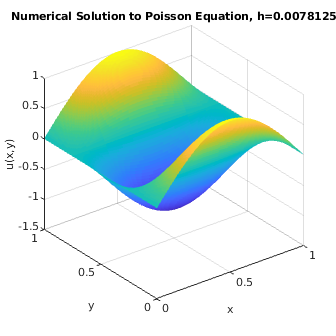
\includegraphics[width=1\linewidth]{hw4_p1_plot}
		%\captionof{figure}{A figure}
		\label{fig:test1}
	\end{minipage}%
	\begin{minipage}{.5\textwidth}
		\centering
		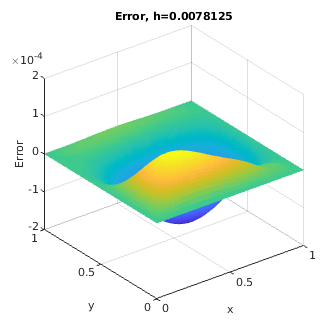
\includegraphics[width=1\linewidth]{hw4_p1_error}
		%\captionof{figure}{Another figure}
		\label{fig:test2}
	\end{minipage}
\end{figure}



\bigbreak
%%%%%%%%%%%%%%%%%%%%%%%%%%%%%%%%%%%%%%%%%%%%%%%%%%%%%%%%%%%%%%%%%%%%%%%%%%%%%%%%%%%%%%%%%%%%%%%%%%%%
\problem{2(a)} Below is my code for solving the Poisson problem on a square domain using sparse matrices.

\begin{lstlisting}[language=MATLAB]
function [u,x,y] = fd2poissonsp(ffun,gfun,a,b,m)
h = (b-a)/(m+1);   % Mesh spacing
[x,y] = meshgrid(a:h:b);   % Uniform mesh, including boundary points.
idx = 2:m+1;
idy = 2:m+1;
% Compute boundary terms, south, north, east, west
ubs = feval(gfun,x(1,1:m+2),y(1,1:m+2));     % Include corners
ubn = feval(gfun,x(m+2,1:m+2),y(m+2,1:m+2)); % Include corners
ube = feval(gfun,x(idy,m+2),y(idy,m+2));     % No corners
ubw = feval(gfun,x(idy,1),y(idy,1));         % No corners
% Evaluate the RHS of Poisson's equation at the interior points.
f = feval(ffun,x(idy,idx),y(idy,idx));
% Adjust f for boundary terms
f(:,1) = f(:,1) - ubw/h^2;             % West
f(:,m) = f(:,m) - ube/h^2;             % East
f(1,1:m) = f(1,1:m) - ubs(idx)/h^2;    % South
f(m,1:m) = f(m,1:m) - ubn(idx)/h^2;    % North
f = reshape(f,m*m,1);
% Create the D2x and D2y matrices
% Full matrix version. Can be made faster with Matlab's sparse library.
%z = [-2;1;zeros(m-2,1)];
z = ones(m,1)*[1 -2 1];
D2 = spdiags(z, [-1 0 1], m, m);
D2x = 1/h^2*kron(D2,speye(m));
D2y = 1/h^2*kron(speye(m),D2);
% Solve the system
u = (D2x + D2y)\f;
% Convert u from a column vector to a matrix to make it easier to work with
% for plotting.
u = reshape(u,m,m);
% Append on to u the boundary values from the Dirichlet condition.
u = [ubs;[ubw,u,ube];ubn];
end
\end{lstlisting}

\bigbreak
%%%%%%%%%%%%%%%%%%%%%%%%%%%%%%%%%%%%%%%%%%%%%%%%%%%%%%%%%%%%%%%%%%%%%%%%%%%%%%%%%%%%%%%%%%%%%%%%%%%%
\problem{2(b)} I have downloaded the MATLAB functions specified.

\bigbreak
%%%%%%%%%%%%%%%%%%%%%%%%%%%%%%%%%%%%%%%%%%%%%%%%%%%%%%%%%%%%%%%%%%%%%%%%%%%%%%%%%%%%%%%%%%%%%%%%%%%%
\problem{2(c)} The results of my timings are given below. These results come from running on my office computer:
\begin{table}[H]
	\caption{System Specifications}
	\begin{center}
		\begin{tabular}{|r|l|}
			\hline
			Make & Dell\\ \hline
			Processor & Intel Core i5-2400 \ \  3.10GHz x 4\\ \hline
			Memory & 7.7GiB $\approx$ 8 GB\\ \hline
			OS & Ubuntu 18.04 - Bionic Beaver\\ \hline
			Application & MATLAB - R2018a \\ \hline
		\end{tabular}
	\end{center}
\end{table}

My computer did not have enough memory to run the dense GE solver for $k=7$. Based on information from \texttt{top} - the default command line resource monitor on ubuntu (and many other systems) - it looks like my system was using around 117\% of the available memory when running this case. My system was using swap space (virtual memory) to complete the script which was dramatically increasing the runtimes. \bigbreak

The wall-clock times for GE when $k \geq 7$ are predicted times. I reasoned that GE is $\mathcal{O}(n^3)$ or in this case $\mathcal{O}((m^2)^3)$, so I did a cubic regression on $m^2$ and the wall-clock time to extrapolate. Since I needed four points for a cubic regression I also included $k=3$.

%\color{gray}
\begin{table}[H]
	\caption{Average Wall-clock time in seconds of 10 runs. {\color{gray}(predicted)}}
	\begin{center}
		\begin{tabular}{|c|c|c|c|c|c|c|}
			\hline
			$k$&$m^2$&GE&SOR&Sparse GE&DST&Multigrid\\ \hline
			3&49&0.0006967&0.0008175&0.0004143&0.0003157&0.0019262\\ \hline
			4&225&0.0037434&0.0023273&0.0007004&0.0003316&0.0030616\\ \hline
			5&961&0.018593&0.0078251&0.0015111&0.0004459&0.0052118\\ \hline
			6&3969&0.57195&0.052586&0.0056945&0.0009885&0.009997\\ \hline
			7&16129&\color{gray}41.263&0.44997&0.027005&0.0020163&0.026672\\ \hline
			8&65025&\color{gray}2808.4&4.2597&0.12434&0.0061616&0.078019\\ \hline
			9&2.6112e+05&\color{gray}1.8377e+05&38.512&0.67354&0.0324&0.41839\\ \hline
			10&1.0465e+06&\color{gray}1.1862e+07&531.5&3.0856&0.13551&2.385\\ \hline
		\end{tabular}
	\end{center}
\end{table}

\bigbreak
%%%%%%%%%%%%%%%%%%%%%%%%%%%%%%%%%%%%%%%%%%%%%%%%%%%%%%%%%%%%%%%%%%%%%%%%%%%%%%%%%%%%%%%%%%%%%%%%%%%%
\problem{2(d)} It should be noted that these predicted times for GE should be taken with a grain of salt for several reasons. Firstly, using only four points for a cubic regression and extrapolating this far outside of the range of the data is generally not going to produce meaningful results. Additionally, technical details of the hardware implementation can have great effect on the wall-clock time. In particular, solving this problem for $k=3 \implies m^2 = 49$ points probably only requires one transfer to the L1 cache. On the other hand the larger values of $k$ will require many page swaps from memory to the caches at best and in my case disk write/reads for virtual memory access. The only meaningful conclusion from these \textit{predicted} data is an example of cubic growth on $m^2$. Though the particular predicted wall-clock time for $k=10$ is not a reliable estimate, that it is roughly in the millions of seconds (weeks!) is significant. \bigbreak

Next I would like to address the seemingly poor performance of SOR. This particular implementation used MATLAB level looping to perform the updates, which is far slower than comparable operations in the libraries that MATLAB uses for vector operations and solving systems. Perhaps the rate of increase of the wall-clock times is significant, but I would not consider this an apples-to-apples comparison with the last three methods. \bigbreak

These points seem moot given the astounding speeds of the Discrete Sine Transform and Multigrid. Since the DST has order $\mathcal{O}(n\log n)) = \mathcal{O}(m^2 \log m ))$ it was expected to be among the fastest. Though Multigrid was slower it is still very impressive, particularly for an iterative method.

\bigbreak
%%%%%%%%%%%%%%%%%%%%%%%%%%%%%%%%%%%%%%%%%%%%%%%%%%%%%%%%%%%%%%%%%%%%%%%%%%%%%%%%%%%%%%%%%%%%%%%%%%%%
\problem{3(a)} Develop a second-order-accurate FD method for solving the Poisson equation on a square with the Neumann boundary conditions that specify zero flux over the boundary. \bigbreak

The system will be the same as in problem 2, with the Dirichlet boundary conditions except for the equations corresponding to points on the boundary. The equations corresponding to the stencils at the corners of the domain are 
%South-West corner (centered at $(x_0,y_0)$) will be 
\begin{align*}
\begin{bmatrix}&2&\\0&-4&2\\&0&\end{bmatrix}u =& f(x_0,y_0) + \frac{4}{h} \sigma(x_0, y_0) \tag{South-West} \\
\begin{bmatrix}&2&\\2&-4&0\\&0&\end{bmatrix}u =& f(x_{m+1},y_0) + \frac{4}{h} \sigma(x_{m+1}, y_0) \tag{South-East} \\
\begin{bmatrix}&0&\\0&-4&2\\&2&\end{bmatrix}u =& f(x_0,y_{m+1}) + \frac{4}{h} \sigma(x_0, y_{m+1}) \tag{North-West} \\
\begin{bmatrix}&0&\\2&-4&0\\&2&\end{bmatrix}u =& f(x_{m+1},y_{m+1}) + \frac{4}{h} \sigma(x_{m+1}, y_{m+1}) \tag{North-East} \\
\end{align*} 
For each other point on the boundary the equations corresponding to the stencils are
%boundary $(x_j, y_0)$ (not including the corners) the equation corresponding to the stencil is
\begin{align*}
%\begin{bmatrix}&1&\\1&-4&1\\&2&\end{bmatrix}u = f(x_0,y_0) + \frac{2}{h} \sigma(x_i, y_0)
\begin{bmatrix}&2&\\1&-4&1\\&0&\end{bmatrix}u =& f(x_i,y_0) + \frac{2}{h} \sigma(x_i, y_0) \tag{Southern} \\
\begin{bmatrix}&1&\\2&-4&0\\&1&\end{bmatrix}u =& f(x_{m+1},y_j) + \frac{2}{h} \sigma(x_{m+1}, y_j) \tag{Eastern} \\
\begin{bmatrix}&0&\\1&-4&1\\&2&\end{bmatrix}u =& f(x_i,y_{m+1}) + \frac{2}{h} \sigma(x_i, y_{m+1}) \tag{Northern} \\
\begin{bmatrix}&1&\\0&-4&2\\&1&\end{bmatrix}u =& f(x_{m+1},y_j) + \frac{2}{h} \sigma(x_{m+1}, y_j) \tag{Western} \\
\end{align*}
In all eight of these cases the stencil center is centered at the point at which $f$ is evaluated. \bigbreak

Since the flux at the boundary is defined to be zero for our problem, in our implementation we ignore the sigma terms. Then we can represent our system of equations at the matrix equation
$$
D_2U + U D_2 = h^2F
$$
Where $D_2$ is the one dimensional second order accurate Finite difference matrix with Neumann boundary conditions, $U$ is our matrix of unknowns, and $F$ the matrix with entries $f(x_i,y_i)$. Applying the DCT (in matrix form $C$) row-wise and column-wise we have
\begin{align*}
CD_2 C^{-1} CUC^{-1} + CUC^{-1} CD_2C^{-1} &= h^2C F C^{-1} \\
\Lambda \hat{U} + \hat{U} \Lambda &= \hat{F} \\
\frac{h^2}{\lambda_{i} + \lambda_{j}} \hat{F}_{i,j} &= \hat{U}_{i,j}.
\end{align*}
The matrix $\Lambda = CD_2C^{-1}$ is diagonal, and the diagonal entries are known giving the key equation
\begin{align}
\hat{U}_{i,j} &= \frac{h^2}{2\cos(\frac{\pi i}{m+1}) + 2\cos(\frac{\pi j}{m+1})-4}\hat{F}_{i,j} \label{keyEquation}
\end{align}
for all values of $\hat{U}$ except for $\hat{U}_{0,0}$ which we choose arbitrarily, and is interpreted as the "total mass" or "total energy" of the solution. Solutions of our PDE will be equivalent up to a constant which corresponds to this value (in general it is not equal). \bigbreak

Thus our full algorithm is almost exactly the same as in our one-dimensional case.
\begin{enumerate}
	\item Form the matrix $F$ where $F_{i,j} = f(x_i, y_j)$.
	\item Compute $\hat{F} = CFC^{-1}$. In implementation this is the DCT applied to the rows and the IDCT (which is equivalent to the DCT up to scaling) to the columns. 
	\item Use (\ref{keyEquation}) to compute $\hat{U}$.
	\item Arbitrarily assign a value corresponding to the total mass $\hat{U}_{0,0}$.
	\item Compute $U = C^{-1}\hat{U}C$. In implementation this is the IDCT applied to the rows, then the DCT applied to the columns.
\end{enumerate}
I have implemented this algorithm in Python, seen below.

\begin{lstlisting}[language=Python]
def fd2poissondct(forcing, a, b, m):
	h = (b-a)/(m+1)
	xs = np.linspace(a, b, m+2)
	X, Y = np.meshgrid(xs, xs)
	fs = foo(X, Y)
	# fhat=(S*f)*S^(-1)
	f_hat = fft.idct(fft.dct(fs, type=1, axis=0)/2,
			type=1, axis=1)/(m+1)
	cos_vec = np.cos(np.pi*np.arange(0,m+2)/(m+1))
	denom = 2*(np.add.outer(cos_vec, cos_vec)-2)
	denom[0,0] = 1 #temporary to allow for the division
	u_hat = h**2 * f_hat / denom
	u_hat[0,0] = 0 # arbitrarily chosen
	us = fft.dct(fft.idct(u_hat, type=1, axis=0)/(m+1),
			type=1, axis=1)/2
	return us
\end{lstlisting}

\bigbreak
%%%%%%%%%%%%%%%%%%%%%%%%%%%%%%%%%%%%%%%%%%%%%%%%%%%%%%%%%%%%%%%%%%%%%%%%%%%%%%%%%%%%%%%%%%%%%%%%%%%%
\problem{3(b)} The fast DCT solver above was applied to the problem with the forcing term of 
$$
f(x,y) = -8\pi^2 \cos(2\pi x )\cos(2\pi y )
$$
for which the exact solution is known analytically. Using $m=2^6-1$ we obtain a relative error in the solution of $\approx 0.000803578$. The solution and error plots can be seen below.
\begin{figure}[H]
	\centering
	\caption{Plots of the solution and error using DCT.}
	\begin{minipage}{.5\textwidth}
		\centering
		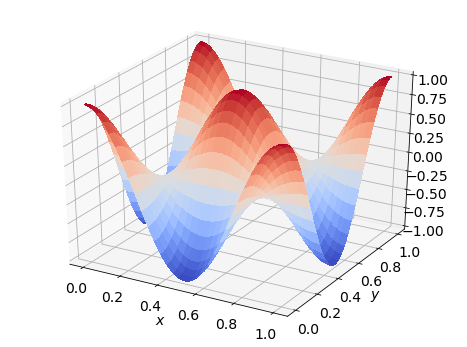
\includegraphics[width=1\linewidth]{hw4_p3_plot}
		%\captionof{figure}{A figure}
		\label{fig:test1}
	\end{minipage}%
	\begin{minipage}{.5\textwidth}
		\centering
		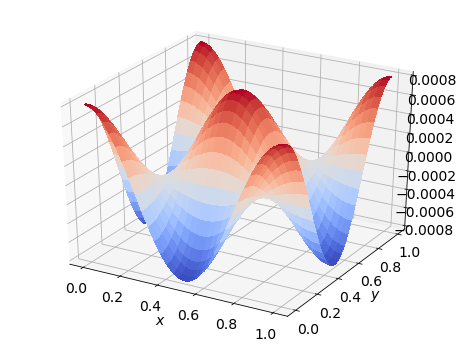
\includegraphics[width=1\linewidth]{hw4_p3_error}
		%\captionof{figure}{Another figure}
		\label{fig:test2}
	\end{minipage}
\end{figure}

This was tested for $m^2-1$ interior points for values of $k=4, 5, ..., 10$. The results are shown in the table below. The table clearly shows that as $m$ doubles (nearly doubles that is) i.e. the step size is halved, the error is reduced by a factor of 4. This suggests second order convergence as we expected.

\begin{center}
	\begin{tabular}{|c|c|c|c|}
		\hline
		$k$&$m=2^k-1$&Relative $L^2$ Error&ratio\\ \hline
		4&15&0.012951&-\\ \hline
		5&31&0.003219&4.0233\\ \hline
		6&63&0.00080358&4.0058\\ \hline
		7&127&0.00020082&4.0014\\ \hline
		8&255&5.0201e-05&4.0004\\ \hline
		9&511&1.255e-05&4.0001\\ \hline
		10&1023&3.1375e-06&4\\ \hline
	\end{tabular}
\end{center}

\bigbreak
%%%%%%%%%%%%%%%%%%%%%%%%%%%%%%%%%%%%%%%%%%%%%%%%%%%%%%%%%%%%%%%%%%%%%%%%%%%%%%%%%%%%%%%%%%%%%%%%%%%%
\problem{4(a)} Our goal is to derive the fourth-order-accurate approximation to $\Delta u = f$:
$$
\frac{1}{6h^2}\begin{bmatrix}1 & 4 & 1\\4 & -20&4\\1&4&1\end{bmatrix}u = \frac{1}{12}\begin{bmatrix} & 1 & \\1 & 8&4\\&1&\end{bmatrix}f + \mathcal{O}(h^4).
$$
To do this, we will need the following three approximations.\\
\textit{Second order approximation to $\Delta f$}:
$$
\Delta f = \frac{1}{h^2}\begin{bmatrix}&1&\\1&-4&1\\&1&\end{bmatrix}f + \mathcal{O}(h^2)
$$

\textit{Fourth order approximation to $\Delta u$}:
\begin{align}
\Delta u = \frac{1}{12h^2}\begin{bmatrix}&&-1&&\\&&16&&\\-1&16&-60&16&-1\\&&16&&\\&&-1&&\end{bmatrix}u + \mathcal{O}(h^4) \label{fourthOrder}
\end{align}

\textit{Second order approximation to $\Delta^2 u$}:
$$
\Delta^2 u = \frac{1}{h^4}\begin{bmatrix}&&1&&\\&2&-8&2&\\1&-8&20&-8&1\\&2&-8&2&\\&&1&&\end{bmatrix}u + \mathcal{O}(h^2)
$$

This last approximation can be seen by applying the Laplacian stencil recursively. That is
\begin{align*}
	\phantom{=}& \frac{1}{h^2}\left( \frac{1}{h^2}\begin{bmatrix}&&1&&\\&1&-4&1&\\&&\color{blue}1&&\\&&&&\\&&&&\end{bmatrix} +
	\frac{1}{h^2}\begin{bmatrix}&&&&\\&1&&&\\1&-4&\color{blue}1&&\\&1&&&\\&&&&\end{bmatrix} +
	\frac{1}{h^2}\begin{bmatrix}&&&&\\&&&1&\\&&\color{blue}1&-4&1\\&&&1&\\&&&&\end{bmatrix} \right.\\
	& \phantom{==}+
	\frac{1}{h^2}\begin{bmatrix}&&&&\\&&&&\\&&\color{blue}1&&\\&1&-4&1&\\&&1&&\end{bmatrix} 
	-4 \frac{1}{h^2} 
	\left. \begin{bmatrix}&&&&\\&&1&&\\&1&\color{blue}-4&1&\\&&1&&\\&&&&\end{bmatrix}
	\right)u + \mathcal{O}(h^2)= \Delta^2 u.
\end{align*}
Here the centers of the stencils have been printed in {\color{blue}blue} so that the relative position is clear. \bigbreak

We first apply the Laplacian to both sides of our PDE to obtain $\Delta^2 u = \Delta f$ and then apply our second order approximations to each side to obtain
\begin{align}
	\frac{1}{h^4}\begin{bmatrix}&&1&&\\&2&-8&2&\\1&-8&20&-8&1\\&2&-8&2&\\&&1&&\end{bmatrix}u & = 
	\frac{1}{h^2}\begin{bmatrix}&1&\\1&-4&1\\&1&\end{bmatrix}f + \mathcal{O}(h^2) \label{secondOrder}
\end{align}

Summing (\ref{fourthOrder}) + $\frac{h^2}{12}$(\ref{secondOrder}) we have
\begin{align*}
	\frac{1}{12h^2}\begin{bmatrix}2&-8&2\\-8&-40&-8\\2&-8&2\end{bmatrix}u &= 
	\frac{1}{12}\begin{bmatrix}&1&\\1&8&1\\&1&\end{bmatrix}f + \mathcal{O}(h^4)\\
	\frac{1}{6h^2}\begin{bmatrix}1 & 4 & 1\\4 & -20&4\\1&4&1\end{bmatrix}u &=
	\frac{1}{12}\begin{bmatrix} & 1 & \\1 & 8&4\\&1&\end{bmatrix}f + \mathcal{O}(h^4)
\end{align*}
as desired.

\bigbreak
%%%%%%%%%%%%%%%%%%%%%%%%%%%%%%%%%%%%%%%%%%%%%%%%%%%%%%%%%%%%%%%%%%%%%%%%%%%%%%%%%%%%%%%%%%%%%%%%%%%%
\problem{4(b)} The Python function below implements this scheme, and solves the system using sparse matrices.

\begin{lstlisting}[language=python]
def fd2_poisson_compact(forcing, boundary, a, b, m):
	h = (b-a)/(m+1)
	diagonals = [4.0, -20, 4]
	main_diag_val = sp.diags(diagonals, [-1,0,1], 
			shape=(m,m), format='csr')
	main_diag_loc = sp.eye(m)
	diagonals = [1, 4, 1]
	sub_diag_val = sp.diags(diagonals, [-1,0,1], 
			shape=(m,m), format='csr')
	sub_diag_loc = sp.diags([1,0,1], [-1, 0, 1], 
			shape=(m,m), format='csr')
	M = sp.kron(main_diag_val, main_diag_loc) 
			+ sp.kron(sub_diag_val, sub_diag_loc)
	
	xs = np.linspace(a,b,m+2, endpoint=True)
	X,Y = np.meshgrid(xs,xs)
	fs = forcing(X,Y)
	us = boundary(X,Y)
	us[1:-1,1:-1] = np.zeros((m,m))
	
	rhs = np.zeros((m,m))
	# sum fs
	rhs +=   fs[1:-1,  :-2] # North
	rhs +=   fs[1:-1, 2:  ] # South
	rhs +=   fs[2:  , 1:-1] # East
	rhs +=   fs[:-2 , 1:-1] # West
	rhs += 8*fs[1:-1, 1:-1] # Center
	rhs *= h**2/2
	# account for boundary conditions
		# corners
	rhs_b = np.zeros((m,m))
	rhs_b += us[:-2,  :-2] # North-west
	rhs_b += us[:-2, 2:  ] # North-east
	rhs_b += us[2: ,  :-2] # South-west
	rhs_b += us[2: , 2:  ] # South-east
		# edges
	rhs_b += 4*us[1:-1,  :-2] # North
	rhs_b += 4*us[1:-1, 2:  ] # South
	rhs_b += 4*us[2:  , 1:-1] # East
	rhs_b += 4*us[:-2 , 1:-1] # West
		#center
	rhs_b += -20*us[1:-1, 1:-1] # Center
	
	rhs -= rhs_b
	rhs = rhs.flatten()
	us[1:-1,1:-1] = spla.spsolve(M,rhs).reshape((m,m))
	return us
\end{lstlisting}

This code was applied to the PDE in problem 2 with $m=2^{10}-1$. The solution and error plots can be seen below.

\begin{figure}[H]
	\centering
	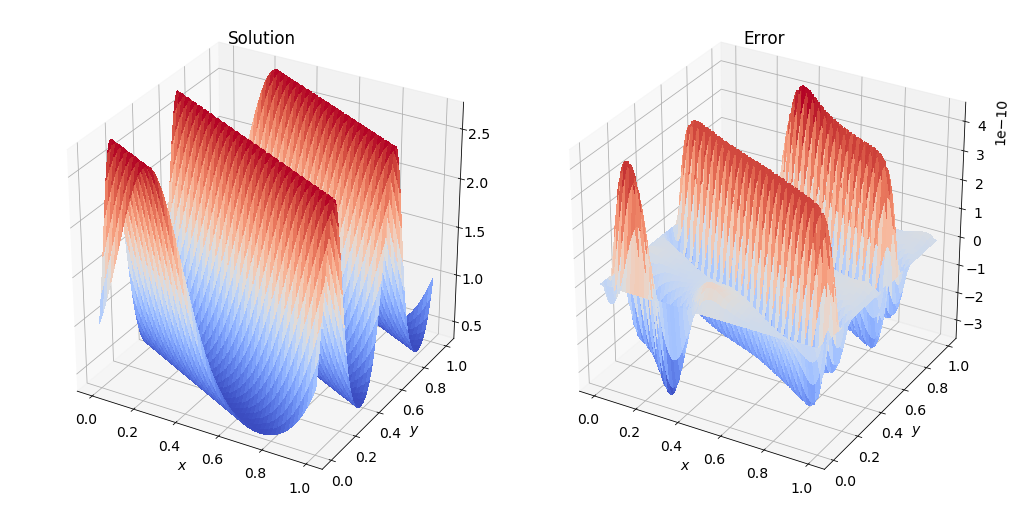
\includegraphics[width=1\linewidth]{hw4_p4}
	%\captionof{figure}{A figure}
\end{figure}

This fourth order algorithm was applied to the PDE in problem 2 with $m=2^k-1$ for $k=4, 5, ..., 10$. The results are seen in the table below and plot. If we refine the mesh by a factor of 2 (roughly double $m$) we see the error go down by a factor of $16=2^4$. This is exactly what we expect from a fourth order algorithm.

\begin{center}
	\begin{tabular}{|c|c|c|c|}
		\hline
		$k$&$m=2^k-1$&Relative $L^2$ Error&ratio\\ \hline
		4&15&0.0021715&-\\ \hline
		5&31&0.0001109&19.58\\ \hline
		6&63&6.6201e-06&16.753\\ \hline
		7&127&4.1065e-07&16.121\\ \hline
		8&255&2.5667e-08&15.999\\ \hline
		9&511&1.6058e-09&15.984\\ \hline
		10&1023&1.0066e-10&15.953\\ \hline
	\end{tabular}
\end{center}

\begin{figure}[H]
	\centering
	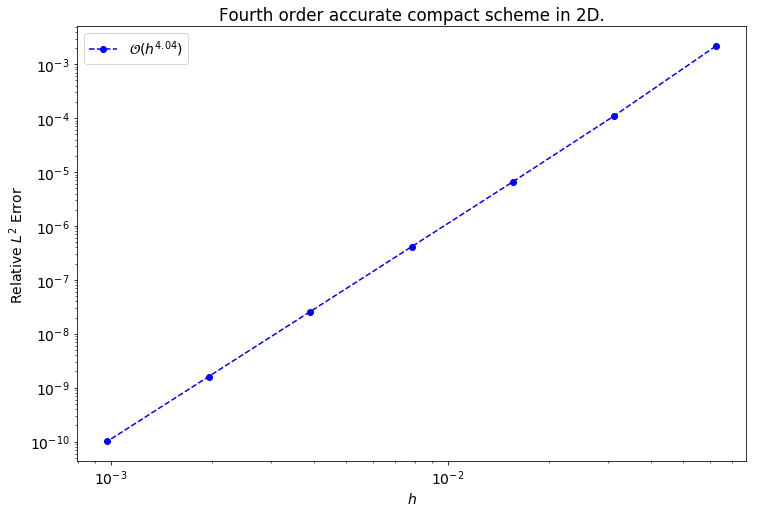
\includegraphics[width=1\linewidth]{hw4_p4_convergence}
	%\captionof{figure}{A figure}
\end{figure}

\bigbreak
%%%%%%%%%%%%%%%%%%%%%%%%%%%%%%%%%%%%%%%%%%%%%%%%%%%%%%%%%%%%%%%%%%%%%%%%%%%%%%%%%%%%%%%%%%%%%%%%%%%%
\problem{4(c)} \textit{Extra Credit} Solve the system from part (b) using the DST. Plot the difference between this solution and the solution from the sparse solver to show that they are essentially the same. Show the computational efficiency. \bigbreak

The key to this algorithm is determining the correct denominator with which to divide $\hat{F}$ in order to calculate $\hat{U}$. We begin by considering the stencil
$$
{\color{blue}u_{-1,-1}+u_{-1,1}+u_{1,-1}+u_{1,1}}+ 4({\color{red}u_{0,-1}+u_{0,1}u_{-1,}u_{1,0}}) - 20 u_{0,0}.
$$
Let $\omega = \frac{\pi}{m+1}$. If we apply our stencil at $u_{i,j}$ and apply the DST row-wise and column-wise ((that is, substitute the 2D DST into the linear system) to the {\color{blue}blue} we get (omitting the $\hat{u}$ for brevity)
\begin{align*}
\sum_{k=1}^m\sum_{l=1}^m & \sin(\omega k(i-1))\sin(\omega l(j-1)) \\
					   + & \sin(\omega k(i+1))\sin(\omega l(j-1)) \\
					   + & \sin(\omega k(i-1))\sin(\omega l(j+1)) \\
					   + & \sin(\omega k(i+1))\sin(\omega l(j+1)) \\
\sum_{k=1}^m\sum_{l=1}^m & \left[ \sin(\omega k(i-1)) + \sin(\omega k(i+1)) \right]\\
					   * & \left[ \sin(\omega l(j-1)) + \sin(\omega l(j+1)) \right]\\
\sum_{k=1}^m\sum_{l=1}^m & 2\sin(\omega ki)\cos(\omega k)2\sin(\omega lj)\cos(\omega l) \\
\sum_{k=1}^m\sum_{l=1}^m & 4\sin(\omega ki)\sin(\omega lj) \cos(\omega k)\cos(\omega l).
\end{align*}

If we do the same for the {\color{red}red} we have
\begin{align*}
\sum_{k=1}^m\sum_{l=1}^m & \sin(\omega k(i-1))\sin(\omega lj) \\
					   + & \sin(\omega k(i+1))\sin(\omega lj) \\
					   + & \sin(\omega ki)\sin(\omega l(j+1)) \\
					   + & \sin(\omega ki)\sin(\omega l(j+1)) \\
\sum_{k=1}^m\sum_{l=1}^m & \sin(\omega lj) \left[ \sin(\omega k(i-1)) + \sin(\omega k(i+1)) \right]\\
					   + & \sin(\omega ki) \left[ \sin(\omega l(j-1)) + \sin(\omega l(j+1)) \right] \\
\sum_{k=1}^m\sum_{l=1}^m & \sin(\omega lj) 2\sin(\omega ki) \cos(\omega k) \\
                       + & \sin(\omega ki) 2\sin(\omega lj) \cos(\omega l) \\
\sum_{k=1}^m\sum_{l=1}^m & 4 \sin(\omega ki)\sin(\omega lj)\cos(\omega k)\cos(\omega l)       
\end{align*}
remarkably the same as the {\color{blue}blue}! \bigbreak

Substituting these into the stencil we have
$$
\sin(\omega ki)\sin(\omega lj) 20\sum_{k=1}^m\sum_{l=1}^m \cos(\omega k)\cos(\omega l) - 1.
$$
Applying the IDST to these gives us our denominator
$$
\hat{U}_{kl} = \frac{\frac{6h^2}{12}}{20\cos(\omega k)\cos(\omega l) - 20} \hat{F}_{kl}.
$$
%
%or equivalently (using a trigonometric identity and making a change of indices)
%$$
%\hat{U}_{kl} = \frac{\frac{6h^2}{12}}{20\big(\cos(\omega k) + \cos(\omega l) - 2\big)} \hat{F}_{kl}.
%$$
At least these formula are almost right. When applied to our problem they give a solution that is close to correct. The plot below shows the solution and the error when the output is scaled by a factor of $\frac{10}{6}$. 
\begin{figure}[H]
	\centering
	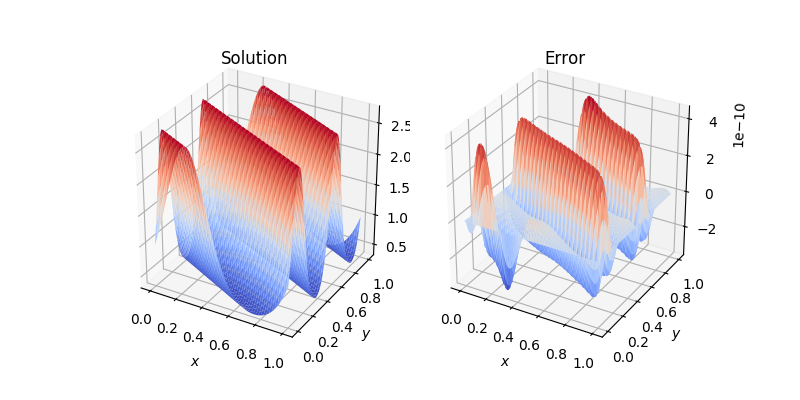
\includegraphics[width=1\linewidth]{hw4_p4_c}
	%\captionof{figure}{A figure}
\end{figure}
It is not clear where this factor comes from, and is likely a mistake in my implementation. Even if the solution were scaled perfectly, the error would not be ideal. It seems that near the boundary the error spikes, particularly at the crests of the waves. Since the adjustments for the boundary conditions are accounted for in the exact same way as the sparse matrix solution it seems very unlikely that this would be the source of the error. More probably the error is in the denominator of the calculation of $\hat{U}$. Specifically the stencils on the boundary have missing values. In the one-dimensional DST these worked out to not be special cases, but to still follow the form. I suspect that having values significantly off of the main diagonal may have some impact on this. I attempted a correction, but was unsuccessful.


\bigbreak
%%%%%%%%%%%%%%%%%%%%%%%%%%%%%%%%%%%%%%%%%%%%%%%%%%%%%%%%%%%%%%%%%%%%%%%%%%%%%%%%%%%%%%%%%%%%%%%%%%%%
\problem{5(a)} Consider the function $f(u,t) = |u|$ on $\mathcal{D}=[-1,1] \times (-\infty, \infty)$. Is $f$ continuous with respect to $u$ on $\mathcal{D}$? \bigbreak

\textit{Claim:} Yes, it is in fact uniformly continuous with respect to $u$. \bigbreak

\begin{proof}
	Let $t \in (-\infty, \infty)$. Let $\delta >0$. Choose $\varepsilon = \delta$. Let $u, u^* \in [-1, 1]$ such that $\vert u - u^* \vert < \delta$. Then 
	\begin{align*}
		\vert f(u, t) - f(u^*,t) \vert &= \big \vert \vert u \vert - \vert u^* \vert \big \vert  \\
		& \leq \vert u - u^* \vert \tag{reverse triangle inequality} \\
		& \leq \delta = \varepsilon.
	\end{align*}
\end{proof}

\bigbreak
%%%%%%%%%%%%%%%%%%%%%%%%%%%%%%%%%%%%%%%%%%%%%%%%%%%%%%%%%%%%%%%%%%%%%%%%%%%%%%%%%%%%%%%%%%%%%%%%%%%%
\problem{5(b)} Is $f$ Lipschitz continuous with respect to $u$ on $\mathcal{D}$? \bigbreak

\textit{Claim:} Yes, it is Lipschitz with constant $L = 1$. \bigbreak

\begin{proof}
	Let $t \in (-\infty, \infty)$. Let $\delta >0$. Choose $\varepsilon = \delta$. Let $u, u^* \in [-1, 1]$ such that $\vert u - u^* \vert < \delta$. Then 
	\begin{align*}
		\vert f(u, t) - f(u^*,t) \vert &= \big \vert \vert u \vert - \vert u^* \vert \big \vert  \\
		& \leq \vert u - u^* \vert. \tag{reverse triangle inequality}
	\end{align*}
\end{proof}

\bigbreak
%%%%%%%%%%%%%%%%%%%%%%%%%%%%%%%%%%%%%%%%%%%%%%%%%%%%%%%%%%%%%%%%%%%%%%%%%%%%%%%%%%%%%%%%%%%%%%%%%%%%
\problem{5(c)} Is the initial value problem 
$$
u'(t) = \vert u \vert, \phantom{=} -1 \leq t \leq 1, \phantom{=}u(-1)=-1 = u_0
$$
well-posed? \bigbreak

\textit{Claim:} Yes, it is well posed. \bigbreak

\begin{proof}
	The function $f(u,t) = \vert u \vert$ is obviously continuous in $t$. \bigbreak
	
	As stated in part (b), $f(u,t) = \vert u \vert$ is Lipschitz on the domain $\mathcal{D}=[-1,1] \times (-\infty, \infty)$. The same proof can be used to show that it is Lipschitz on $\mathcal{D}=[a,b] \times [-1,1]$ for any closed interval $[a,b]$. \bigbreak
	
	By our Existence and Uniqueness Theorem we have that the IVP has a unique solution for $t \in [-1, 1]$. Lastly we need to show that the solution varies continuously with perturbations of the initial conditions and forcing term. \bigbreak
	
	Let $\varepsilon > 0$ be given. Choose $\kappa (\varepsilon) = 2$. Let $\delta(t)$ be a continuous function, and let $\tilde u_0 \in [-1,1]$ such that $\vert \delta(t) \vert < \varepsilon$ and so that $\vert \tilde u_0 - u_0 \vert < \varepsilon$ and the solution $\tilde u$ to
	$$
	\tilde u' = \vert \tilde u \vert + \delta(t)
	$$
	exists. \bigbreak
	
	Define $y = \tilde u - u$ and $y_0 = \tilde u_0 - u_0$. Then $y$ satisfies the differential equation
	$y' = \delta(t)$ and $\vert y' \vert < \varepsilon$ with $\vert y_0 \vert < \varepsilon$ as well. So the solution $y = \int_{-1}^t \delta(\tau) d\tau + y_0$ can be bounded by 
	$$
	\varepsilon(-t) - \varepsilon < y < \varepsilon t + \varepsilon
	$$
	or simply $\vert y \vert < \varepsilon (\vert t \vert + 1) \leq 2\varepsilon = \kappa(\varepsilon)\varepsilon$. Thus showing that the IVP varies continuously with the initial conditions and forcing term and is therefore well-posed. 
\end{proof}

\end{document}
